\documentclass[11pt]{article}

\usepackage[T1]{fontenc}
\usepackage{lmodern}
\usepackage{amsmath,amssymb,amsthm}
\usepackage[margin=1.15in]{geometry}
\usepackage{microtype}
\usepackage{booktabs}
\usepackage{array}
\usepackage{graphicx}
\usepackage{enumitem}
\usepackage{xcolor}
\usepackage[colorlinks=true,linkcolor=black,citecolor=black,urlcolor=blue!55!black]{hyperref}

\theoremstyle{plain}
\newtheorem{lemma}{Lemma}
\newtheorem{proposition}{Proposition}
\newtheorem{corollary}{Corollary}
\theoremstyle{definition}
\newtheorem{definition}{Definition}
\theoremstyle{remark}
\newtheorem{remark}{Remark}

\newcommand{\KL}{D_{\mathrm{KL}}}
\newcommand{\TV}{d_{\mathrm{TV}}}
\newcommand{\I}{\mathrm{I}}
\newcommand{\Pp}{\mathbb{P}}
\newcommand{\LR}{\operatorname{LR}}
\newcommand{\LRh}{\widehat{\operatorname{LR}}}

\title{Stylometric Proxies}
\author{Flyxion\\\textit{Independent Researcher}}
\date{September 2026}

\begin{document}
\maketitle

\begin{abstract}
Readers increasingly treat visible features of prose, such as em dashes, balanced triads, stock transitions, compressed antitheses, and recurring syntactic frames, as evidence that a text was generated by a language model. Such judgments begin from a real but temporary correlation and convert it into a public test of provenance. Once public, the test changes both populations it purports to distinguish. Model users can suppress a flagged feature at negligible cost, while human writers who use it naturally are pressured to censor or defend their own style. The proxy therefore decouples from authorship while its social cost persists. This essay formalizes that process in three steps. First, mutual information between authorship and a public feature collapses under adaptive convergence, and the collapse is bounded above and below by total variation. Second, in a linear adaptation model the machine population lags the human one, so the feature keeps some evidential value during the transition. Third, readers update their beliefs about the cue more slowly than either population changes its behavior, so believed diagnosticity exceeds actual diagnosticity by an unbounded factor even as both approach the uninformative limit. The essay then reviews precedents in Federalist-era stylometry, adversarial authorship attribution, spam filtering, and search ranking, distinguishes four Goodhart-type failures, and examines where the cost of a bad proxy lands. It argues that provenance should be carried by histories, meaning drafts, timestamps, version logs, and commit trails, rather than inferred from appearance, while conceding that unanchored histories are themselves cheap to fabricate. The defensible alternative is a record anchored to external, time-stamped commitments, which supports claims about priority, order, and continuity but cannot certify the absence of machine assistance.
\end{abstract}

\section{The Inference Chain}

Authorship is not visible in a finished sentence. What a reader sees is an artifact left by a process, and the process is only imperfectly connected to the identity or kind of agent that took part in it. The inferential chain can be written
\[
A \longrightarrow \Pi \longrightarrow T \longrightarrow F,
\]
where $A\in\{H,M\}$ denotes a human or machine provenance class, $\Pi$ the production process, $T$ the completed text, and $F=\phi(T)$ a vector of surface features extracted from it. The final arrow may count punctuation, function words, sentence lengths, syntactic templates, lexical frequencies, or any other measurable regularity. The reader attempts to invert the chain:
\[
F \rightsquigarrow A.
\]
The hooked arrow marks an inference rather than a reversal of causation.

The distinction matters most when the process is composite. A human may dictate a paragraph, ask a model to shorten it, restore two deleted qualifications, and then revise every sentence. A model may generate only an outline. A copy editor may regularize punctuation in a text written without generative assistance. A human may deliberately imitate the cadence attributed to a model, while a model may be instructed to imitate the irregularities attributed to a human. The binary variable $A$ is already a compression of a richer production history, and a surface cue is a second compression applied to the first.

For a single binary feature $f$, such as the presence of a construction above a declared rate, the rational evidential quantity is the likelihood ratio
\[
\LR(f)
=
\frac{\Pp(f\mid A=M)}{\Pp(f\mid A=H)}.
\]
An em dash is not intrinsically machine-like. It counts as evidence only relative to estimated conditional distributions in a specified population, genre, language, model family, prompting regime, and period. The posterior odds are
\[
\frac{\Pp(M\mid f)}{\Pp(H\mid f)}
=
\LR(f)
\frac{\Pp(M)}{\Pp(H)}.
\]
The base rate matters as much as the cue. A feature with a modest likelihood ratio generates many false accusations when machine authorship is uncommon, and the same feature may reverse meaning across genres. The inference commonly made in practice suppresses every qualification in these equations: the reference population, the time index, the genre, the prior odds, the production process, and the uncertainty of the estimates.

The resulting folk detector is simple. Models use em dashes; this text uses em dashes; therefore a model wrote this text. The middle premise is unstable. At best it reports that, at a particular time, some models under some settings used a visible feature at a higher rate than some human comparison set. A population-level difference becomes an individual verdict, and a dated correlation is treated as a permanent signature.

\subsection{What a consequential verdict requires}\label{sec:threshold}

Suppose a reader or institution must decide whether to act on the belief that a text is machine-generated. Let $c_{\mathrm{FP}}$ be the cost of acting against a human author and $c_{\mathrm{FN}}$ the cost of failing to act against a machine text. Acting minimizes expected cost exactly when
\[
\frac{\Pp(M\mid e)}{\Pp(H\mid e)} \;\ge\; \frac{c_{\mathrm{FP}}}{c_{\mathrm{FN}}},
\]
where $e$ is the total evidence. Combined with the posterior-odds identity, this requires a likelihood ratio of at least
\[
\LR^\ast
=
\frac{c_{\mathrm{FP}}}{c_{\mathrm{FN}}}\cdot\frac{1-\pi}{\pi},
\]
with $\pi=\Pp(M)$ the prior probability of machine authorship in the relevant population.

Consider a setting in which one text in five is machine-generated ($\pi=0.2$) and a false accusation is judged ten times as costly as a missed detection. Then $\LR^\ast = 10\cdot 4 = 40$. A single punctuation habit with a likelihood ratio of 2, which is generous for one surface feature, leaves posterior odds of $0.5$: a text bearing the cue still has a two-in-three chance of a human author. The gap between what a surface cue delivers and what a consequential verdict demands is the first reason the proxy cannot bear the weight placed on it. The dynamics of the following sections show that the gap widens over time.

\section{Why the Proxy Formed}

The surface test did not arise from nothing. Early outputs from widely used language models often displayed recognizable regularities: balanced paragraphs, explicit signposting, summary conclusions, antithetical constructions, enumerations in threes, uniformly polished transitions, and a preference for certain words and punctuation marks. A model samples from a learned distribution under decoding and alignment constraints, and a default assistant persona can concentrate stylistic tendencies that are more diffuse in the human corpus from which it learned.

Some of these impressions have been measured. Kobak and colleagues studied vocabulary changes across millions of PubMed abstracts from 2010 to 2024 and found an abrupt rise in the frequency of certain style words after the appearance of ChatGPT-like models \cite{kobak2025}. That result concerns lexical items in one genre and does not by itself establish rates for punctuation or syntactic frames. For the cues most discussed in public, the em dash and the balanced triad, the evidence is thinner and largely anecdotal. The argument of this essay does not need those rates to be large. It needs only that a difference was reported, widely believed, and adopted as a test.

A cue can therefore exist briefly. Let
\[
p_M^{(0)}=\Pp(f=1\mid M),
\qquad
p_H^{(0)}=\Pp(f=1\mid H).
\]
If $p_M^{(0)}>p_H^{(0)}$, observing $f$ raises the posterior probability of $M$. Nothing in the argument requires denying that initial inequality. The difficulty begins when three propositions are collapsed into one:
\begin{enumerate}[label=(\roman*),leftmargin=2.2em]
\item the feature differed in frequency between two sampled populations;
\item the feature remains discriminative after the difference becomes public;
\item the feature warrants a consequential judgment about an individual text.
\end{enumerate}
Only the first follows from the initial observation. The second depends on how the populations respond to publication, which is the subject of Section~\ref{sec:collapse}, and the third depends on the decision threshold of Section~\ref{sec:threshold}.

\subsection{Two routes to convergence}

Publication moves the two conditional distributions toward each other by different mechanisms.

The first route is suppression. ``Do not use em dashes'' is a short instruction, as are ``avoid triadic lists,'' ``vary paragraph length,'' and ``do not use the construction `not X but Y.' '' A cue that can be described in a viral post can generally be described in a prompt. Communicability is the reason a cue spreads as a detector and the reason it is fragile as one. Human suppression is costlier. A writer does not toggle a decoding preference. The marked construction may belong to a practiced rhythm, a disciplinary convention, a second-language register, an accessibility strategy, or a style learned decades before the relevant model existed. Avoiding it can require continuous monitoring and can make the prose less natural to its author. The same public rule therefore imposes unequal modification costs on the two populations.

The second route is absorption. Yakura and colleagues analyzed hundreds of thousands of hours of spoken discourse and report that words preferentially generated by ChatGPT rose abruptly in spontaneous human speech after its release \cite{yakura2025}. If humans adopt machine-preferred vocabulary through exposure or through routine editing assistance, then $p_H$ moves toward $p_M$ from below, and the likelihood ratio approaches one without any human avoidance at all. The formal analysis below treats the direction of human movement as a free parameter, so both routes fall under it. The two routes have opposite consequences for cost. Avoidance imposes a displacement cost on human writers. Absorption may impose none, though it erases whatever stylistic distinctiveness the displaced habits carried.


\section{Precedents and Related Work}\label{sec:precedents}

The argument sits among five literatures that are often treated separately: authorship attribution, adversarial stylometry, adversarial classification in spam and search, machine-generated-text detection, and content provenance. Read together, they describe a change in the evidential environment. Classical attribution asks which comparatively stable habits distinguish known authors. Adversarial work asks whether those habits survive once a writer knows they are being measured. Detection extends the contest to rapidly changing model families and inexpensive rewriting. Provenance systems respond by attaching claims to a recorded production history rather than extracting them from the finished surface.

\subsection{Attribution under stable conditions}

Modern computational stylometry uses lexical, character-level, syntactic, and structural features to distinguish candidate authors. Surveys emphasize that performance depends on the size and genre of the texts, the candidate set, topic control, and the representation chosen \cite{stamatatos2009}. Mosteller and Wallace's analysis of the disputed \emph{Federalist Papers} remains the canonical success \cite{mosteller1963,mosteller1964}. The target was a fixed historical corpus, the candidate authors were known, and the features were function words such as prepositions and conjunctions, which are common, weakly tied to subject matter, and hard for an author to monitor continuously. Their evidential value came from being habitual and, at the time, unavailable as a public optimization target.

The lesson is often summarized as proof that style reveals authorship. A more exact reading is that some distributions of low-salience features can carry authorship information under a stable production regime. Had Hamilton and Madison been handed the attribution model in advance and rewarded for defeating it, the evidential setting would have changed. The analysis succeeded on historical traces, not on outputs generated interactively against its decision rule.

Attribution also differs in form from contemporary folk detection. Attribution ordinarily compares an unknown text with reference writing from particular candidates. The public cue attempts open-world classification between heterogeneous classes called ``human'' and ``machine,'' each containing many styles, tasks, and production arrangements. The second problem has weaker class definitions and faster distribution shift.

Mechanical document examination offers a contrast. A typewriter can leave recurring defects produced by wear, alignment, damaged type, ribbon behavior, and spacing. Such traces belong to the history of a physical inscription, and their evidential force depends on a causal path from a particular mechanism to a particular mark. Calling both practices ``fingerprinting'' hides the distinction. A damaged type slug is evidence of an instrument because the instrument repeatedly causes the mark. An em dash is evidence of, at most, a population-level tendency, because many unrelated processes cause it.

\subsection{Adversarial stylometry and the publication effect}

The stability assumption was challenged well before large language models. Kacmarcik and Gamon gave writers feedback about the features an attribution system used so that they could revise a document toward anonymity \cite{kacmarcik2006}. Brennan, Afroz, and Greenstadt framed obfuscation and imitation as adversarial attacks on authorship recognition \cite{brennan2012}. Later work shows both the promise and the limits of such transformations: obfuscation may lower attribution accuracy yet introduce detectable artifacts of its own \cite{mahmood2020}, and a replication found that some early claims of effectiveness were overstated \cite{wang2022}.

The result that matters here is that publication changes the object of study, whether or not evasion always succeeds. Once a feature set or classifier is known, the observed text is partly a response to the measurement regime. Stylometry becomes a strategic interaction among attributor, author, editor, and transformation system. A public em-dash rule is a crude instance of the same loop.

\subsection{Spam filtering and search ranking}

Spam filtering made the adaptive problem explicit. Statistical filters learned words and structures associated with unwanted mail, and senders responded with ``good word'' attacks, substitutions, images, and other evasions. Research on spam filtering treats the sender as an active adversary rather than a stationary class \cite{bratko2006,jorgensen2008}. A feature does not remain diagnostic merely because it once separated two corpora.

Search ranking followed a parallel course. Keyword frequency and link counts were initially usable indicators of relevance or authority. Once rankings controlled attention and revenue, optimization industries formed around the indicators. Deepak, Steinhoff, and Simoes describe keyword stuffing under content-based search as an instance of adversarial Goodhart and note the suggestion that a robust proxy should be conceptually simple and hard to optimize for \cite{deepak2024}. Keyword stuffing and link farms did not show that the original correlations were fictional. They showed that a correlation used for allocation becomes part of the causal environment it measures. The repeated arc is
\[
\text{correlation}
\longrightarrow
\text{public rule}
\longrightarrow
\text{optimization pressure}
\longrightarrow
\text{distribution shift}
\longrightarrow
\text{proxy decay}.
\]
The pattern has older statements in the social sciences, in Campbell's observation that quantitative indicators used for decisions become subject to corruption pressure \cite{campbell1979} and in Goodhart's remark on statistical regularities under control pressure \cite{goodhart1984}. Stylometric provenance is an unusually rapid instance, because the generator can respond to a newly public rule almost immediately.

\subsection{Generated-text detection, rewriting, and unequal error}

Generated-text detectors use several families of evidence: supervised classifiers, statistical regularities in model probabilities, watermark signals, and human judgment. DetectGPT identifies curvature properties of a model's log-probability function rather than a named punctuation habit \cite{mitchell2023}. Watermarking embeds a statistical signal during generation that a keyed detector can test \cite{kirchenbauer2023}. A recent survey finds a recurring problem across families: robustness must be assessed across models, domains, decoding strategies, attacks, and mixtures of human and machine contribution \cite{wu2025}. The target is not stationary.

Evasion experiments make the problem concrete. Krishna and colleagues found that paraphrasing sharply reduced the performance of several detectors; in one reported setting, their paraphraser reduced DetectGPT's detection rate from 70.3 percent to 4.6 percent at a 1 percent false-positive rate \cite{krishna2023}. Their proposed defense retrieves passages from a database of previously generated text rather than relying on the current passage's appearance, which already moves from appearance toward history. Sadasivan and colleagues give complementary empirical and theoretical reasons to doubt reliable detection under unrestricted adaptation \cite{sadasivan2023}. These studies do not show that every detector is useless. They show that performance on a fixed benchmark does not establish durable provenance inference after transformation.

The fairness literature identifies a second failure mode. Liang and colleagues found that several detectors frequently classified essays by non-native English writers as machine-generated and that generated text could be prompted to evade detection \cite{liang2023}. Distributional difference is therefore an allocation question as well as an accuracy question. When the positive label carries suspicion, heterogeneous false-positive rates assign the social cost of uncertainty to particular groups of human writers.

\subsection{What the literatures leave open}

These literatures establish four pieces of the argument: style can be informative under controlled conditions; knowledge of the test induces strategic rewriting; detectors are vulnerable to transformation and distribution shift; and errors can be unequally distributed. Three pieces are missing. The first is a single temporal claim joining them, in which a public surface proxy begins with genuine likelihood-ratio evidence, loses information as both conditional distributions adapt, and leaves a positive human adjustment cost. The second is an account of the reader, whose beliefs about a cue change on their own schedule and need not track the cue's actual diagnosticity. The third is a candid treatment of the proposed alternative, since history-based evidence faces the same adaptive pressures. Sections~\ref{sec:collapse}, \ref{sec:records}, and~\ref{sec:cost} address these in turn.

\section{Goodhart Dynamics}\label{sec:goodhart}

Manheim and Garrabrant distinguish four families of Goodhart effects: regressional, extremal, causal, and adversarial \cite{manheim2019}. Stylometric provenance cues exhibit all four, though not equally well. Table~\ref{tab:goodhart} states where each mapping is close and where it strains.

\begin{table}[ht]
\centering
\small
\renewcommand{\arraystretch}{1.25}
\begin{tabular}{@{}>{\raggedright\arraybackslash}p{0.13\textwidth}>{\raggedright\arraybackslash}p{0.44\textwidth}>{\raggedright\arraybackslash}p{0.33\textwidth}@{}}
\toprule
Variant & Mechanism for a stylistic cue & Fit \\
\midrule
Regressional & A cue chosen for looking strongly diagnostic in an early sample regresses toward its true effect on a broader sample. & Close. \\
Extremal & The cue is applied to genres and individual texts outside the region where its relation to authorship was estimated. & Loose. The mechanism is domain shift rather than optimization pushed to extremes. \\
Causal & Penalizing the cue treats a symptom of a production regime as if it were the regime. & Close for confounded cues such as formal register. \\
Adversarial & Anyone who gains from evasion, or whose text is mislabeled, adapts to the public rule. & Close. Includes the reflexive shift in the human population. \\
\bottomrule
\end{tabular}
\caption{Mapping of the four Goodhart variants onto stylometric cues.}
\label{tab:goodhart}
\end{table}

\subsection{Regressional failure}

A feature selected because it looked unusually diagnostic in an early sample combines signal with noise. Selection favors features whose observed separation was inflated by sampling variation, topical imbalance, model-version effects, or an accident of the comparison corpus. Measured again on a broader population, the apparent effect regresses toward its underlying value. The cue may still correlate with provenance, but less dramatically than its public reputation suggests.

\subsection{Extremal failure}

Even a reliable average difference need not survive extrapolation to individual texts or unusual genres. A detector calibrated on student essays may be applied to legal prose, grant applications, technical documentation, or translated fiction. In those regions the causal mixture producing the feature changes. Formulaic structure can arise from genre constraints rather than machine generation, and low lexical variability can reflect language proficiency rather than synthetic origin. This variant is the weakest fit to the Manheim and Garrabrant taxonomy, since no one is optimizing the proxy toward extreme values in the ordinary sense. The mechanism is closer to covariate shift, and the label is kept only because the practical consequence is the same: the proxy is carried outside the region in which its relation to the target was estimated.

\subsection{Causal failure}

The feature may correlate with machine output because both are consequences of a third variable such as formal register, constrained vocabulary, aggressive copy editing, rubric compliance, or a prompt requesting clarity. Penalizing the feature does not remove machine authorship. It removes one visible effect of the production regime, and the intervention leaves the target untouched.

\subsection{Adversarial failure}

Once a cue is used to deny credit, assign blame, reject submissions, or trigger investigation, anyone who benefits from evasion has an incentive to suppress it. Authorship obfuscation research formalizes this setting, with an attributor and an author or transformer adapting against one another \cite{mahmood2020}. Work on generated-text detection likewise shows that paraphrasing can defeat multiple detectors, including statistical and watermark-based approaches \cite{krishna2023,sadasivan2023}. The adversarial variant also covers the reflexive effect that many discussions file under causal failure: if readers punish em dashes, human writers use fewer of them, which changes the denominator of the original likelihood ratio. The measurement policy becomes a cause of the distribution it later claims merely to observe.

\subsection{Cue stacking}

Readers rarely rely on one cue. A text with an em dash, a balanced triad, and an antithetical frame seems to bear three independent marks. A naive reader combines them as
\[
\log\text{odds}_{\text{naive}}
=
\log\frac{\pi}{1-\pi}+\sum_{i=1}^{k}\log\LR(f_i),
\]
which is valid only when the cues are conditionally independent given provenance. They rarely are, because a shared register or genre tends to produce them together. Take two binary cues with $\Pp(f_i{=}1\mid H)=0.3$ and $\Pp(f_i{=}1\mid M)=0.6$. If the cues are independent within each class, the joint likelihood ratio for seeing both is $(0.6)^2/(0.3)^2=4$. If a single latent register drives both, so that within each class they co-occur perfectly, seeing both is exactly as informative as seeing one, and the joint likelihood ratio is $0.6/0.3=2$. The naive product overstates the evidence by a factor of two in this example, and the overstatement grows geometrically with the number of correlated cues. The perceived strength of a pattern of cues is therefore inflated in precisely the cases, formal and heavily edited prose, where the cues co-occur for benign reasons.

\subsection{Interaction}

The failures compound. A noisily selected cue is publicized; it is applied beyond its calibration domain; publication causes conscientious humans to avoid it; generators remove it adversarially; and stacked cues inflate the apparent strength of what remains. The result is a moving target whose movement was partly caused by the diagnostic itself, and not a degraded but otherwise stationary test.

\section{Information Collapse and Persistent Cost}\label{sec:collapse}

The mathematical claim is narrower than the slogan that every public test becomes useless. Publicity alone does not imply convergence. A costly physical assay can remain informative after its operation is known, and a stylistic feature may stay discriminative if one population cannot or will not change it. The collapse result requires adaptive convergence as an assumption. This section states the assumption, derives it from an explicit adaptation model, and then adds a third ingredient, the reader's beliefs, which turns loss of information into a persistent burden.

\subsection{Information and total variation}

Let $P_H^t$ and $P_M^t$ be the distributions of a public feature vector $F_t$ at time $t$ conditional on human and machine provenance, and let $\pi\in(0,1)$ be the prior probability of machine provenance. The mutual information between authorship and the feature is
\[
\I_t(A;F)
=
\pi\,\KL\!\left(P_M^t\,\middle\|\,\bar P^t\right)
+(1-\pi)\,\KL\!\left(P_H^t\,\middle\|\,\bar P^t\right),
\qquad
\bar P^t=\pi P_M^t+(1-\pi)P_H^t,
\]
the prior-weighted Jensen--Shannon divergence between the two conditional distributions. Information is measured in nats unless a table says bits. Write $\TV(P,Q)=\tfrac12\int|p-q|$ for total variation.

\begin{lemma}[Information and total variation]\label{lem:tv}
For every $\pi\in(0,1)$ and every pair of distributions $P_M,P_H$,
\[
2\pi(1-\pi)\,\TV(P_M,P_H)^2
\;\le\;
\I(A;F)
\;\le\;
2\max(\pi,1-\pi)\,\TV(P_M,P_H).
\]
\end{lemma}

The lower bound is a Pinsker-type inequality and the upper bound follows from a chi-square bound on each divergence term; both are proved in Appendix~\ref{app:proofs}. Their consequence is that, for fixed $\pi$, information vanishes exactly when total variation does. The hypothesis of the next result therefore states precisely the behavior that the model of Section~\ref{sec:dynamics} derives.

\begin{proposition}[Collapse with persistent cost]\label{prop:collapse}
Suppose a publicly known stylometric test induces adaptation such that $\TV(P_M^t,P_H^t)\to 0$. Then $\I_t(A;F)\to0$. Suppose in addition that human adaptation converges to a distribution $P_H^\infty$ different from the pre-publication baseline $P_H^0$, and that changing style carries a strictly positive human cost, $C_H(P_H^\infty,P_H^0)>0$, for as long as the displacement persists. Then the feature loses asymptotic information about provenance while imposing a positive cost on human writers in the limit.
\end{proposition}

\begin{proof}
The first claim is immediate from the upper bound of Lemma~\ref{lem:tv}. The second claim does not follow from information collapse alone. It follows from the persistence assumption, since a limiting human distribution displaced from its baseline with strictly positive cost of displacement gives $C_H(P_H^\infty,P_H^0)>0$ while the limiting provenance information is zero.
\end{proof}

The proposition is deliberately modest, since both of its substantive premises are assumptions. The next two subsections replace them with derived statements.

\subsection{A model of adaptation}\label{sec:dynamics}

For a stylized binary feature, let $p_H^t$ and $p_M^t$ be the human and machine usage rates after round $t$. Suppose public suspicion moves human writers toward a ``safe'' rate $s\in(0,1)$, while machine operators cheaply track the most recently observed human rate:
\begin{align}
p_H^{t+1} &= (1-\alpha)\,p_H^t+\alpha\, s,\label{eq:human}\\
p_M^{t+1} &= (1-\beta)\,p_M^t+\beta\, p_H^t,\label{eq:machine}
\end{align}
with $0<\alpha,\beta<1$. Write $a=p_H^0-s$ for the initial human displacement and $d_t=p_M^t-p_H^t$ for the machine excess. For a binary feature $\TV(P_M^t,P_H^t)=|d_t|$. Let human adjustment cost be $C_H^t=\kappa_H\,(p_H^t-p_H^0)^2$ with $\kappa_H>0$.

\begin{proposition}[Adaptation dynamics]\label{prop:dyn}
Under \eqref{eq:human} and \eqref{eq:machine}:
\begin{enumerate}[label=(\alph*),leftmargin=2.2em]
\item $p_H^t=s+a(1-\alpha)^t$, and $p_M^t\to s$.
\item If $\alpha\ne\beta$,
\[
d_t=(1-\beta)^t d_0+a\alpha\,\frac{(1-\beta)^t-(1-\alpha)^t}{\alpha-\beta},
\]
and if $\alpha=\beta$, $d_t=(1-\beta)^t d_0+a\alpha\,t(1-\alpha)^{t-1}$.
\item $d_t=O(t\rho^t)$ with $\rho=\max(1-\alpha,1-\beta)$, so $\TV(P_M^t,P_H^t)\to0$ and, by Lemma~\ref{lem:tv}, $\I_t(A;f)\to0$ at the same geometric rate.
\item If $a\ge0$ and $d_0>0$ (humans move away from the feature while the machine starts above them), then $d_t>0$ for every $t$, so $\LR_t=1+d_t/p_H^t>1$ throughout: the machine lags, and the feature keeps positive but vanishing evidential value during the transition.
\item $C_H^t=\kappa_H a^2\bigl(1-(1-\alpha)^t\bigr)^2\to\kappa_H a^2$, which is positive whenever $a\neq0$.
\end{enumerate}
\end{proposition}

Part (d) is a refinement worth stating. The public rule does not become useless at the moment it is announced. It decays along a path on which the machine population trails the human one. Part (e) records the cost side: the human displacement is complete in the limit, and the cost is positive as long as nothing induces humans to move back.

\begin{remark}
The likelihood ratio and the information are different quantities. In the illustration below, $\LR_t$ rises slightly in the first rounds while $\I_t$ falls monotonically, because the feature also becomes rarer among humans. Information is small for a rare cue even when its ratio is high, and a reader who consults only the ratio will overestimate how much the cue can still tell them.
\end{remark}

\subsection{Belief lag}\label{sec:belief}

The propositions so far describe the two writing populations. The harm to human writers passes through a third population, the readers, whose beliefs about a cue need not track its current diagnosticity. Suppose readers estimate the feature rates by exponential smoothing of what they observe,
\begin{equation}
q_H^{t+1}=(1-\gamma)\,q_H^t+\gamma\,p_H^t,
\qquad
q_M^{t+1}=(1-\gamma)\,q_M^t+\gamma\,p_M^t,
\label{eq:belief}
\end{equation}
with $0<\gamma<1$ and calibrated initial beliefs $q^0=p^0$. The believed likelihood ratio is $\LRh_t=q_M^t/q_H^t$. A reader who sees the feature assigns machine probability
\[
\hat\phi_t=\frac{\pi\,q_M^t}{\pi\,q_M^t+(1-\pi)\,q_H^t},
\]
whereas the calibrated value uses the true rates and is $\phi^\ast_t=\pi p_M^t/(\pi p_M^t+(1-\pi)p_H^t)$. Both tend to $\pi$ when the rates coincide, and both are increasing in the respective likelihood ratio.

\begin{proposition}[Belief lag]\label{prop:belief}
Under \eqref{eq:human}, \eqref{eq:machine}, and \eqref{eq:belief}:
\begin{enumerate}[label=(\alph*),leftmargin=2.2em]
\item $q_H^t\to s$ and $q_M^t\to s$.
\item If $d_t\ge0$ for all $t$, the believed excess $\Delta_t=q_M^t-q_H^t$ satisfies $\Delta_t\ge(1-\gamma)^t d_0$.
\item If in addition $a\ge0$, $d_0>0$, and $\gamma<\min(\alpha,\beta)$, then
\[
\frac{\LRh_t-1}{\LR_t-1}\longrightarrow\infty,
\]
and consequently $\hat\phi_t>\phi^\ast_t$ for all sufficiently large $t$, while both tend to $\pi$.
\end{enumerate}
\end{proposition}

Part (c) is the sense in which readers keep believing after the signal is gone. Both the actual and the believed likelihood ratios tend to one, but the believed excess is larger by an unbounded factor. When readers update more slowly than either writing population adapts, the reader's suspicion of a feature-bearing text stays above the calibrated value for a period whose length scales as $1/\gamma$. Human writers pay for that period twice: once by the distributional displacement of part (e) of Proposition~\ref{prop:dyn}, and again by the excess suspicion that attaches to any residual use of the feature.

\subsection{Illustration}

Table~\ref{tab:dyn} and Figure~\ref{fig:dyn} show a run with $p_H^0=0.30$, $p_M^0=0.60$, $s=0.05$, $\alpha=0.30$, $\beta=0.40$, $\gamma=0.10$, and $\pi=0.20$. The parameters are stylized and are not estimates from any corpus. They fix a case in which humans cut their use of the feature from 30 percent of texts to 5 percent, the machine follows with a lag, and readers update more slowly than either writing population.

\begin{table}[ht]
\centering
\small
\begin{tabular}{@{}rccccccc@{}}
\toprule
$t$ & $p_H^t$ & $p_M^t$ & $\operatorname{LR}_t$ & $\widehat{\operatorname{LR}}_t$ & $\I_t$ (bits) & $\phi_t^\ast$ & $\hat\phi_t$ \\
\midrule
0 & 0.300 & 0.600 & 2.00 & 2.00 & 0.0435 & 0.333 & 0.333 \\
2 & 0.172 & 0.378 & 2.19 & 2.01 & 0.0263 & 0.354 & 0.334 \\
4 & 0.110 & 0.232 & 2.11 & 2.03 & 0.0131 & 0.345 & 0.337 \\
8 & 0.064 & 0.100 & 1.55 & 2.01 & 0.0020 & 0.280 & 0.335 \\
12 & 0.053 & 0.063 & 1.18 & 1.93 & 0.0002 & 0.227 & 0.325 \\
16 & 0.051 & 0.053 & 1.05 & 1.81 & 0.0000 & 0.207 & 0.311 \\
24 & 0.050 & 0.050 & 1.00 & 1.52 & 0.0000 & 0.200 & 0.276 \\
32 & 0.050 & 0.050 & 1.00 & 1.29 & 0.0000 & 0.200 & 0.243 \\
\bottomrule
\end{tabular}

\caption{Illustrative run. $\LR_t$ and $\LRh_t$ are the actual and believed likelihood ratios; $\I_t$ is the information between authorship and the feature in bits; $\phi_t^\ast$ and $\hat\phi_t$ are the calibrated and believed probabilities that a feature-bearing text is machine-generated.}
\label{tab:dyn}
\end{table}

\begin{figure}[ht]
\centering
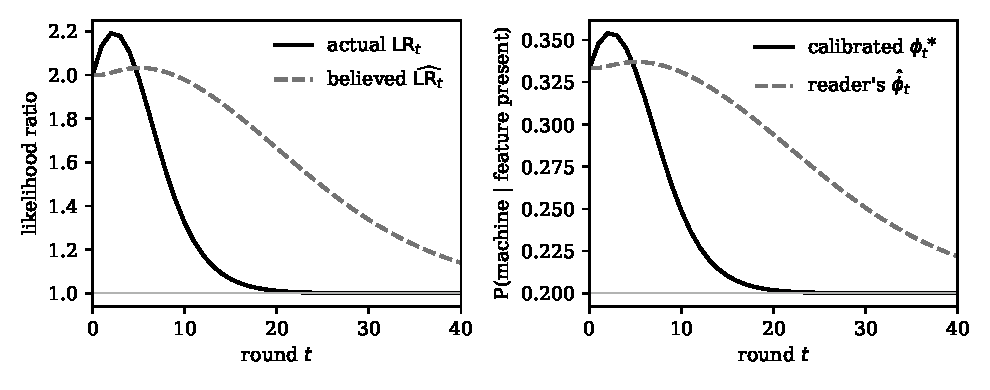
\includegraphics[width=\textwidth]{fig_dynamics.pdf}
\caption{Actual versus believed diagnosticity for the run of Table~\ref{tab:dyn}. Left: likelihood ratios. Right: probability that a feature-bearing text is machine-generated; the horizontal line is the prior $\pi$.}
\label{fig:dyn}
\end{figure}

Three features of the run deserve attention. Information falls monotonically and is negligible by round 12, at which point the actual likelihood ratio is $1.18$ while the believed ratio is still $1.93$. The reader's posterior for a feature-bearing text sits at $0.325$ when the calibrated value has fallen to $0.227$. And at round 32 the actual ratio is one to two decimal places while readers still credit the cue with a ratio of $1.29$, so a residual excess suspicion of about four percentage points persists long after the signal has vanished.

\subsection{Scope of the results}

\begin{remark}
These results are conditional. If machine and human feature distributions do not converge, the feature may retain information. If human writers relax back toward their baseline once suspicion subsides, the cost of part (e) of Proposition~\ref{prop:dyn} is transient, and its duration inherits the belief lag of Proposition~\ref{prop:belief}, since humans respond to perceived rather than actual suspicion. In the absorption case, with $a<0$, the sign conclusions of part (d) change, while parts (a) through (c) hold. The cost asymmetry can be represented by $\kappa_H\gg\kappa_M$, which is not a claim that all human stylistic change is painful or that all machine control is free. A model operator can often change a named surface feature through a one-line constraint, whereas a human writer may have to inspect each sentence, abandon habitual punctuation, or accept suspicion. The machine-side cost is paid once as an instruction, and the human-side cost recurs as attention.
\end{remark}

\section{Where the Cost Falls}\label{sec:cost}

The immediate victim of a weak proxy is the person whose authorship is questioned. A model has no reputation to defend, no educational record to correct, and no attachment to an em dash. The accused writer may be asked to produce drafts, explain vocabulary, reproduce the work under observation, or accept a lowered evaluation because a reader has mistaken resemblance for provenance.

\subsection{Heterogeneity among human writers}

Variation within the human population sharpens the asymmetry. Liang and colleagues tested several widely used detectors on essays written by native and non-native English writers. The detectors frequently misclassified the latter as machine-generated while performing much better on the native-writer comparison set \cite{liang2023}. Their experiments also showed that prompting could alter generated text enough to reduce detection, so both sides of the asymmetry appear in one study: constrained human expression attracted suspicion while machine output adapted around it.

The result should not be inflated into the claim that every later detector shows the same measured bias. It establishes a structural possibility in prominent systems: a detector can attach suspicion to features of constrained linguistic variation that arise for reasons other than machine generation. No malicious design is required. The error arises when a feature with heterogeneous human causes is treated as if it had one technological cause.

The same structure appears for folk rules, and it can be stated exactly. Let writers of group $g$ use the feature at natural rate $p_g$, and let readers assign machine probability $\hat\phi$ to any feature-bearing text. The suspicion borne by a writer of group $g$ per text is $p_g\hat\phi$, so for two groups the ratio of burdens is
\[
\frac{p_g\,\hat\phi}{p_{g'}\,\hat\phi}=\frac{p_g}{p_{g'}},
\]
independent of how strongly readers believe in the cue. A uniform belief therefore produces a proportionally unequal burden, and a group whose members also face a high avoidance cost $\kappa_g$ pays twice. Non-native writers, formal writers, and heavily edited writers are the groups most likely to combine a high natural rate with a high avoidance cost.

\subsection{Decision thresholds}

Section~\ref{sec:threshold} showed that a consequential verdict requires posterior odds above the cost ratio. In the setting used there, with $\pi=0.2$ and $c_{\mathrm{FP}}/c_{\mathrm{FN}}=10$, action requires a posterior machine probability of roughly $0.91$. The believed posterior in the illustration of Table~\ref{tab:dyn} never exceeds $0.34$, and the calibrated posterior never exceeds $0.36$. A surface cue can justify a question to the author. On these numbers it cannot justify a sanction, and the belief-lag result shows that the gap between the sanction readers feel entitled to impose and the sanction the evidence supports widens over time before it narrows.

\subsection{A self-sealing judgment}

Once a cue has been noticed, ordinary examples become confirming instances. A reader who has learned that ``AI uses tricolons'' does not calculate uncertainty, since the rule changes perception. The accused writer occupies an awkward evidential position: removing the feature can be read as concealment, retaining it as confirmation, and protesting the inference as defensiveness. A defeasible cue becomes a self-sealing social judgment.

\subsection{Pre-emptive flattening}

A further cost is hypothesized here rather than measured. Writers who are never accused may still trade preferred punctuation for punctuation believed to be safe, replace useful transitions with awkward ones, or add deliberate roughness as a certificate of humanity. If so, the resulting register is detector-facing prose, optimized to avoid resembling a public caricature of machine prose. The proposition of Section~\ref{sec:collapse} supplies the structure of such a cost, and an empirical test would compare within-writer usage rates before and after the cue became publicly known.

\section{Records as Evidence}\label{sec:records}

If surface appearance becomes least trustworthy exactly when provenance matters most, provenance should be carried by a different object. A better list of forbidden punctuation is the wrong remedy. The candidate is a history. This section develops the case and then states the limits of the case, since a history is exposed to the same adaptive pressures as a style.

\subsection{Logs and rendering}

A completed document supplies one visible state. A version history supplies a trajectory
\[
T_0 \rightarrow T_1 \rightarrow \cdots \rightarrow T_n.
\]
Timestamps, diffs, notes, source citations, recorded experiments, compiler outputs, and commits do not prove that every transformation was performed without assistance. They expose a sequence of commitments. A reader can see when a claim entered, what it replaced, which evidence caused a revision, and whether the final object is continuous with an earlier line of work.

This is the distinction developed in \emph{Commitment Before Appearance} \cite{flyxion2026}: one visible artifact is compatible with many incompatible histories, one log can be folded into several appearances, and similar appearances can arise from different logs. Let $L=(T_0,\Delta_1,\ldots,\Delta_n)$ denote a development log and let $\rho(L)=T_n$ be the rendering map that returns the final text. Since $\rho$ is many-to-one, inversion from $T_n$ to $L$ is generally impossible:
\[
\rho(L_1)=\rho(L_2)
\;\nRightarrow\;
L_1=L_2.
\]
A stylometric proxy attempts precisely this unavailable inversion. It reads a property of $T_n$ and assigns a production history. A provenance record retains part of $L$ before rendering erases it.

\subsection{Records are proxies too}

The argument of Sections~\ref{sec:goodhart} and~\ref{sec:collapse} applies to records once they become public tests. A commit history, a set of dated drafts, or a screenshot of an editor is a feature vector extracted from the process, and its evidential value depends on the cost of producing it without the process. That cost varies enormously across record types. An unsigned list of draft dates can be typed in an afternoon. A version history held by a platform that permits backfilling can be edited. An agentic system can generate a plausible sequence of small commits, with realistic messages and revisions, faster than a human can read them. If ``has a commit trail'' became the new public test, ceremonial trails would follow, and the essay's own dynamics would predict the same decay from information to burden, with human writers who keep no logs bearing the cost.

The right comparison, then, is between records of different forgery cost, and the claim is comparative. Spence's analysis of signaling supplies the relevant principle: a signal carries information to the extent that its cost differs across the types it is meant to separate \cite{spence1973}. A style cue, once known, has a nearly zero cost differential, since a model pays one instruction and a human pays attention. A record can retain a cost differential only if producing it requires something the forger cannot supply after the fact.

\subsection{Anchoring}

\begin{definition}[Anchored record]
A record of a production history is \emph{anchored} to the extent that producing, after a time $t$, a record indistinguishable from it to a verifier requires a resource that cannot be obtained after $t$: elapsed wall-clock time, a commitment previously made to an external party, or a key whose custody is independently attested.
\end{definition}

The simplest anchor is a timestamped digest. Haber and Stornetta's construction places a hash of a document into an append-only, publicly witnessed log \cite{haber1991}.

\begin{proposition}[Priority by anchored digest]\label{prop:anchor}
Let $H$ be a hash function that is preimage-resistant and collision-resistant. Suppose a digest $\delta$ is recorded in a public append-only log at time $t$. Then, except with negligible probability, any document $D$ presented later with $H(D)=\delta$ is the document from which $\delta$ was computed, and the party who submitted $\delta$ possessed $D$ no later than $t$.
\end{proposition}

\begin{proof}[Sketch]
Computing $\delta=H(D)$ requires $D$ or a preimage of $\delta$, which preimage resistance makes infeasible to find after the fact for a value chosen in advance. A different document $D'\neq D$ with $H(D')=\delta$ would be a collision. The log fixes the time at which $\delta$ was committed and cannot be rewritten by the submitter.
\end{proof}

A chain of such digests $\delta_0,\ldots,\delta_n$ committed at times $t_0<\cdots<t_n$ gives a verifier an ordered, externally dated sequence of versions. The forgery cost has a specific shape. Producing the chain after an accusation is impossible for any interval that has already passed, because the commitments would have had to be made then. This blocks on-demand fabrication in response to a challenge. It does not block pre-emptive fabrication: an operator can run many synthetic histories in parallel, each accruing digests in real time. Anchoring therefore raises the barrier for the case that matters most for individual accusation, a fast after-the-fact reconstruction, and leaves mass pre-emptive forgery about as costly per history as elapsed time and no more.

Signed manifests address a different problem. A content-provenance manifest of the kind specified by the Coalition for Content Provenance and Authenticity records signed claims about creation, editing actions, assets, and timestamps \cite{c2pa2025}. Its own specification is careful about the limit: a valid signature authenticates the claim and the signer, and it does not establish that every assertion is true. Trust moves from the surface of the text to the custody of the signing key and the reputation of the signer, which is a more tractable object of scrutiny than a punctuation habit.

\subsection{What records can and cannot establish}

An honest treatment states the strongest claim each kind of evidence supports. Anchored records can establish priority (a version existed by a given time), order (versions appeared in a given sequence), continuity (a later version is a modification of an earlier one, so a claimed line of work developed over a claimed span), and accountability (a named party stands behind a claim). They cannot establish the absence of machine assistance, since a model can operate in real time within an honestly anchored process. Table~\ref{tab:evidence} summarizes the comparison.

\begin{table}[ht]
\centering
\small
\renewcommand{\arraystretch}{1.25}
\begin{tabular}{@{}>{\raggedright\arraybackslash}p{0.21\textwidth}>{\raggedright\arraybackslash}p{0.22\textwidth}>{\raggedright\arraybackslash}p{0.17\textwidth}>{\raggedright\arraybackslash}p{0.28\textwidth}@{}}
\toprule
Evidence & Cost to fabricate after an inquiry & Burden on an honest writer & What it can establish \\
\midrule
Surface cue & One instruction & High if the cue is a natural habit & A population-level tendency at one date \\
Unsigned draft list or screenshot & Low & Low & That some material existed \\
Platform edit history & Moderate, depends on who can edit & Low & Sequence as the platform reports it \\
Signed manifest & Depends on key custody & Low to moderate & That a signer asserts claims, not that they are true \\
Externally anchored digest chain & At least the claimed elapsed time & Low, automatable & Priority, order, and continuity, not absence of assistance \\
\bottomrule
\end{tabular}
\caption{Comparison of evidence types by forgery cost, burden, and scope.}
\label{tab:evidence}
\end{table}

The consequence is a change in the question asked. The relevant inquiry often is whether a named party can stand behind a body of work and show that it developed as claimed. Whether a model touched a sentence is frequently the wrong question, and no available evidence can answer it in general. Records answer the first question well and the second only partially.

\subsection{Commit before reveal}

A low-cost practice follows. A writer who wishes to preserve the option of establishing provenance can publish digests of successive versions to an external append-only service and reveal the underlying drafts only if a claim is challenged. The digests disclose nothing about content, so privacy and the right to discard drafts are preserved, and the marginal cost is a scripted call. The practice supplies the anchor of the previous subsection without requiring anyone to publish a surveillance archive of composition.

\subsection{The burden problem, again}

Because records can become the next public test, the essay's own analysis prescribes guardrails. Absence of a log must be read as uncertainty, since treating it as evidence of machine authorship would reproduce the asymmetry that afflicts the em dash: writers who informally draft, write on paper, or discard drafts would bear the cost. Requests for records should be reserved for consequential decisions. Because the belief-lag result shows that readers hold on to cues after they fail, any institution that adopts a record-based standard should schedule its review, so that the standard is retired or revised when its forgery cost falls.

\subsection{Practice for readers and institutions}

The analysis yields a short set of working rules.
\begin{enumerate}[label=(\arabic*),leftmargin=2.2em]
\item Treat a surface cue as a reason to ask a question and never as a finding.
\item State the stakes and the cost ratio $c_{\mathrm{FP}}/c_{\mathrm{FN}}$ in advance, and compute the likelihood ratio the decision requires.
\item Do not combine correlated cues as if they were independent.
\item Where a consequential decision depends on provenance, ask for anchored records and treat their absence as uncertainty.
\item Audit any cue-based procedure for differential error across writer groups, in particular non-native and formal writers.
\item Review cue-based procedures on a schedule, since the likelihood ratio of a public cue decays and beliefs about it decay more slowly.
\end{enumerate}

\section{Conclusion}

Stylometric proxies begin in observation and end in governance. Someone notices a surface difference, the difference is compressed into a rule, and readers begin allocating trust through it. From that moment the feature no longer merely describes. It changes how models are prompted, how humans write, and who must prove that their sentences belong to them.

The central failure is temporal. A cue measured before publication is applied after publication as though the populations had stayed fixed, while the public test enters both production processes. Models can be instructed around it, and writers can be disciplined by it. Under adaptive convergence the information carried by the cue tends to zero, and the linear model shows that the approach is gradual, with the machine population trailing the human one. Readers update their beliefs more slowly still, so believed diagnosticity exceeds actual diagnosticity by an unbounded factor as both vanish. Human displacement persists for as long as readers' beliefs do.

The resulting detector is inverted. It is cheapest for the system it is meant to detect and costliest for the people it falsely resembles. Non-native writers, formal writers, heavily edited writers, and anyone whose natural cadence overlaps the current stereotype inherit the cost of maintaining a distinction that adaptation has already eroded.

Style still matters. It can reveal genre, training, convention, audience, imitation, and sometimes authorship. What it cannot bear is the full weight of provenance after its features have become public tests. A history of transformations and commitments can carry more of that weight, provided the history is anchored to something the forger cannot supply after the fact, and provided its limits are stated. Records establish priority, order, continuity, and accountability. They leave open whether a model took part, and no honest evidence closes that question. Institutions that need an answer to it should ask for the record that fits the claim, and they should treat the missing record as an open question rather than a verdict.

\appendix

\section{Proofs}\label{app:proofs}

\subsection{Proof of Lemma~\ref{lem:tv}}

Write $p_M,p_H$ for densities with respect to a common measure and $\bar p=\pi p_M+(1-\pi)p_H$. Then $p_M-\bar p=(1-\pi)(p_M-p_H)$ and $p_H-\bar p=-\pi(p_M-p_H)$.

\emph{Lower bound.} By Pinsker's inequality, $\KL(P\|Q)\ge2\,\TV(P,Q)^2$. Since $\TV(P_M,\bar P)=(1-\pi)\TV(P_M,P_H)$ and $\TV(P_H,\bar P)=\pi\,\TV(P_M,P_H)$,
\[
\I\ge 2\pi(1-\pi)^2\,\TV^2+2(1-\pi)\pi^2\,\TV^2=2\pi(1-\pi)\,\TV^2.
\]

\emph{Upper bound.} From $\log x\le x-1$, $\KL(P\|Q)\le\chi^2(P\|Q)=\int (p-q)^2/q$. Applying this to each term with $Q=\bar P$,
\[
\I\le\pi(1-\pi)^2X+(1-\pi)\pi^2X=\pi(1-\pi)X,
\qquad
X=\int\frac{(p_M-p_H)^2}{\bar p}.
\]
Let $m=\min(\pi,1-\pi)$. Then $\bar p\ge m(p_M+p_H)\ge m|p_M-p_H|$, so $X\le m^{-1}\int|p_M-p_H|=2\,m^{-1}\TV$. Since $\pi(1-\pi)/m=\max(\pi,1-\pi)$, the bound $\I\le2\max(\pi,1-\pi)\,\TV$ follows. \qed

\subsection{Proof of Proposition~\ref{prop:dyn}}

(a) Equation \eqref{eq:human} is a linear recurrence with fixed point $s$, giving $p_H^t-s=(1-\alpha)^t a$. Then \eqref{eq:machine} averages a convergent sequence with itself, so $p_M^t\to s$.

(b) Subtracting \eqref{eq:human} from \eqref{eq:machine},
\[
d_{t+1}=(1-\beta)d_t+\alpha\,(p_H^t-s)=(1-\beta)d_t+\alpha a(1-\alpha)^t.
\]
Unrolling gives $d_t=(1-\beta)^td_0+\alpha a\sum_{k=0}^{t-1}(1-\beta)^{t-1-k}(1-\alpha)^k$. The sum equals $\bigl((1-\beta)^t-(1-\alpha)^t\bigr)/(\alpha-\beta)$ when $\alpha\ne\beta$ and $t(1-\alpha)^{t-1}$ when $\alpha=\beta$.

(c) With $x=1-\beta$ and $y=1-\alpha$, the mean value theorem gives $|x^t-y^t|/|x-y|\le t\max(x,y)^{t-1}$. Hence $|d_t|\le|d_0|\rho^t+|a|\alpha\,t\rho^{t-1}$, which is $O(t\rho^t)$ for $\rho>0$ and vanishes for $\rho=0$. Lemma~\ref{lem:tv} converts this to a bound on $\I_t$.

(d) If $a\ge0$ then $p_H^t-s=a(1-\alpha)^t\ge0$, so $d_{t+1}=(1-\beta)d_t+\alpha(p_H^t-s)\ge(1-\beta)d_t>0$ by induction from $d_0>0$.

(e) By (a), $p_H^t-p_H^0=a\bigl((1-\alpha)^t-1\bigr)$, and squaring gives the stated cost. \qed

\subsection{Proof of Proposition~\ref{prop:belief}}

(a) Equation \eqref{eq:belief} is exponential smoothing of a sequence converging to $s$, which converges to $s$.

(b) Subtracting the two smoothing equations gives $\Delta_{t+1}=(1-\gamma)\Delta_t+\gamma d_t$. If $d_t\ge0$ then $\Delta_{t+1}\ge(1-\gamma)\Delta_t$, and $\Delta_0=d_0$ by the calibrated start, so $\Delta_t\ge(1-\gamma)^td_0$.

(c) By the bound in the proof of Proposition~\ref{prop:dyn}(c), $d_t\le d_0\rho^t+a\alpha\,t\rho^{t-1}$ with $\rho=1-\min(\alpha,\beta)<1-\gamma$. Hence $d_t/(1-\gamma)^t\to0$ (trivially if $\rho=0$), and by (b), $\Delta_t/d_t\to\infty$. Now $\LRh_t-1=\Delta_t/q_H^t$ and $\LR_t-1=d_t/p_H^t$, so
\[
\frac{\LRh_t-1}{\LR_t-1}=\frac{\Delta_t}{d_t}\cdot\frac{p_H^t}{q_H^t}\longrightarrow\infty,
\]
because $p_H^t/q_H^t\to1$ when $s>0$. Since $\LR_t-1>0$, eventually $\LRh_t>\LR_t$, and $\hat\phi_t>\phi^\ast_t$ follows from monotonicity of the posterior in the likelihood ratio. Both tend to $\pi$ because both ratios tend to one. \qed

\begin{thebibliography}{99}

\bibitem{brennan2012}
M. Brennan, S. Afroz, and R. Greenstadt,
``Adversarial Stylometry: Circumventing Authorship Recognition to Preserve Privacy and Anonymity,''
\emph{ACM Transactions on Information and System Security}, vol. 15, no. 3, article 12, 2012.
doi: \href{https://doi.org/10.1145/2382448.2382450}{10.1145/2382448.2382450}.

\bibitem{bratko2006}
A. Bratko, G. V. Cormack, B. Filipi\v{c}, T. R. Lynam, and B. Zupan,
``Spam Filtering Using Statistical Data Compression Models,''
\emph{Journal of Machine Learning Research}, vol. 7, pp. 2673--2698, 2006.

\bibitem{c2pa2025}
Coalition for Content Provenance and Authenticity,
\emph{C2PA Technical Specification}, version 2.4, 2026.
\url{https://spec.c2pa.org/specifications/specifications/2.4/specs/C2PA_Specification.html}.

\bibitem{campbell1979}
D. T. Campbell,
``Assessing the Impact of Planned Social Change,''
\emph{Evaluation and Program Planning}, vol. 2, no. 1, pp. 67--90, 1979.

\bibitem{deepak2024}
Deepak P, J. Steinhoff, and S. Simoes,
``On the Political Economy of Link-based Web Search,''
arXiv: \href{https://arxiv.org/abs/2404.16530}{2404.16530}, 2024.

\bibitem{flyxion2026}
Flyxion,
``Commitment Before Appearance,'' unpublished manuscript, 2026.

\bibitem{goodhart1984}
C. A. E. Goodhart,
\emph{Monetary Theory and Practice: The UK Experience}.
London: Macmillan, 1984.

\bibitem{haber1991}
S. Haber and W. S. Stornetta,
``How to Time-Stamp a Digital Document,''
\emph{Journal of Cryptology}, vol. 3, no. 2, pp. 99--111, 1991.

\bibitem{jorgensen2008}
Z. Jorgensen, Y. Zhou, and M. Inge,
``A Multiple Instance Learning Strategy for Combating Good Word Attacks on Spam Filters,''
\emph{Journal of Machine Learning Research}, vol. 9, pp. 1115--1146, 2008.

\bibitem{kacmarcik2006}
G. Kacmarcik and M. Gamon,
``Obfuscating Document Stylometry to Preserve Author Anonymity,''
in \emph{Proceedings of the COLING/ACL 2006 Main Conference Poster Sessions}, pp. 444--451, 2006.
\url{https://aclanthology.org/P06-2058/}.

\bibitem{kirchenbauer2023}
J. Kirchenbauer, J. Geiping, Y. Wen, J. Katz, I. Miers, and T. Goldstein,
``A Watermark for Large Language Models,''
in \emph{Proceedings of the 40th International Conference on Machine Learning}, PMLR vol. 202, pp. 17061--17084, 2023.

\bibitem{kobak2025}
D. Kobak, R. Gonz\'alez-M\'arquez, E.-\'A. Horv\'at, and J. Lause,
``Delving into LLM-assisted Writing in Biomedical Publications through Excess Vocabulary,''
\emph{Science Advances}, 2025. arXiv: \href{https://arxiv.org/abs/2406.07016}{2406.07016}.

\bibitem{krishna2023}
K. Krishna, Y. Song, M. Karpinska, J. Wieting, and M. Iyyer,
``Paraphrasing Evades Detectors of AI-Generated Text, but Retrieval Is an Effective Defense,''
in \emph{Advances in Neural Information Processing Systems}, vol. 36, 2023.
arXiv: \href{https://arxiv.org/abs/2303.13408}{2303.13408}.

\bibitem{liang2023}
W. Liang, M. Yuksekgonul, Y. Mao, E. Wu, and J. Zou,
``GPT Detectors Are Biased Against Non-Native English Writers,''
\emph{Patterns}, vol. 4, no. 7, 100779, 2023.
doi: \href{https://doi.org/10.1016/j.patter.2023.100779}{10.1016/j.patter.2023.100779}.

\bibitem{mahmood2020}
A. Mahmood, Z. Shafiq, and P. Srinivasan,
``A Girl Has a Name: Detecting Authorship Obfuscation,''
arXiv: \href{https://arxiv.org/abs/2005.00702}{2005.00702}, 2020.

\bibitem{manheim2019}
D. Manheim and S. Garrabrant,
``Categorizing Variants of Goodhart's Law,''
arXiv: \href{https://arxiv.org/abs/1803.04585}{1803.04585}, revised 2019.

\bibitem{mitchell2023}
E. Mitchell, Y. Lee, A. Khazatsky, C. D. Manning, and C. Finn,
``DetectGPT: Zero-Shot Machine-Generated Text Detection Using Probability Curvature,''
in \emph{Proceedings of the 40th International Conference on Machine Learning}, PMLR vol. 202, pp. 24950--24962, 2023.
\url{https://proceedings.mlr.press/v202/mitchell23a.html}.

\bibitem{mosteller1963}
F. Mosteller and D. L. Wallace,
``Inference in an Authorship Problem: A Comparative Study of Discrimination Methods Applied to the Authorship of the Disputed Federalist Papers,''
\emph{Journal of the American Statistical Association}, vol. 58, no. 302, pp. 275--309, 1963.

\bibitem{mosteller1964}
F. Mosteller and D. L. Wallace,
\emph{Inference and Disputed Authorship: The Federalist}.
Reading, MA: Addison-Wesley, 1964.

\bibitem{sadasivan2023}
V. S. Sadasivan, A. Kumar, S. Balasubramanian, W. Wang, and S. Feizi,
``Can AI-Generated Text Be Reliably Detected?''
arXiv: \href{https://arxiv.org/abs/2303.11156}{2303.11156}, 2023.

\bibitem{spence1973}
M. Spence,
``Job Market Signaling,''
\emph{Quarterly Journal of Economics}, vol. 87, no. 3, pp. 355--374, 1973.

\bibitem{stamatatos2009}
E. Stamatatos,
``A Survey of Modern Authorship Attribution Methods,''
\emph{Journal of the American Society for Information Science and Technology}, vol. 60, no. 3, pp. 538--556, 2009.
doi: \href{https://doi.org/10.1002/asi.21001}{10.1002/asi.21001}.

\bibitem{wang2022}
H. Wang, P. Juola, and A. Riddell,
``Reproduction and Replication of an Adversarial Stylometry Experiment,''
arXiv: \href{https://arxiv.org/abs/2208.07395}{2208.07395}, 2022.

\bibitem{wu2025}
J. Wu, S. Yang, R. Zhan, Y. Yuan, L. S. Chao, and D. F. Wong,
``A Survey on LLM-Generated Text Detection: Necessity, Methods, and Future Directions,''
\emph{Computational Linguistics}, vol. 51, no. 1, 2025.
\url{https://aclanthology.org/2025.cl-1.8/}.

\bibitem{yakura2025}
H. Yakura, E. Lopez-Lopez, L. Brinkmann, I. Serna, P. Gupta, I. Soraperra, and I. Rahwan,
``Empirical Evidence of Large Language Model's Influence on Human Spoken Communication,''
arXiv: \href{https://arxiv.org/abs/2409.01754}{2409.01754}, 2024, rev. 2025.

\end{thebibliography}

\end{document}
